% Template for Cogsci submission with R Markdown

% Stuff changed from original Markdown PLOS Template
\documentclass[10pt, letterpaper]{article}

\usepackage{cogsci}
\usepackage{pslatex}
\usepackage{float}
\usepackage{caption}

% amsmath package, useful for mathematical formulas
\usepackage{amsmath}

% amssymb package, useful for mathematical symbols
\usepackage{amssymb}

% hyperref package, useful for hyperlinks
\usepackage{hyperref}

% graphicx package, useful for including eps and pdf graphics
% include graphics with the command \includegraphics
\usepackage{graphicx}

% Sweave(-like)
\usepackage{fancyvrb}
\DefineVerbatimEnvironment{Sinput}{Verbatim}{fontshape=sl}
\DefineVerbatimEnvironment{Soutput}{Verbatim}{}
\DefineVerbatimEnvironment{Scode}{Verbatim}{fontshape=sl}
\newenvironment{Schunk}{}{}
\DefineVerbatimEnvironment{Code}{Verbatim}{}
\DefineVerbatimEnvironment{CodeInput}{Verbatim}{fontshape=sl}
\DefineVerbatimEnvironment{CodeOutput}{Verbatim}{}
\newenvironment{CodeChunk}{}{}

% cite package, to clean up citations in the main text. Do not remove.
\usepackage{cite}

\usepackage{color}

% Use doublespacing - comment out for single spacing
%\usepackage{setspace}
%\doublespacing


% % Text layout
% \topmargin 0.0cm
% \oddsidemargin 0.5cm
% \evensidemargin 0.5cm
% \textwidth 16cm
% \textheight 21cm

\title{Should I learn or should I make it go? ~Balancing informational and
social goals in active learning}


\author{{\large \bf Erica J. Yoon*}, {\large \bf Kyle MacDonald*}, {\large \bf Mika Asaba}, {\large \bf Hyowon Gweon}, \and {\large \bf Michael C. Frank} \\ \{ejyoon, kylem4, masaba, hyo, mcfrank\} @stanford.edu \\ Department of Psychology, Stanford University \\ *These authors contributed equally to this work.}

\begin{document}

\maketitle

\begin{abstract}
Our actions shape what we learn. Empirical and theoretical work shows
that people are capable of efficient self-directed learning to maximize
informational goals. But a fundamental feature of human learning is that
it unfolds within a social context. How can we begin to understand the
role of social factors in self-directed learning? Here, we present a
computational model that integrates the value of social and information
goals to predict the decisions that people will make in a simple active
causal learning task. We show that emphasizing performance or
self-presentation goals leads to actions that reduce the chances of
learning (E1). Next, we show that the presence of an observer (i.e., a
boss) pushes learners to emphasize performance/presentation actions even
when emphasis is placed on a learning goal (E2). Our formal model of
social-active learning successfully captured key patterns in the
empirical results. These findings represent an important first step
towards integrating active learning with social reasoning.

\textbf{Keywords:}
active learning; social reasoning; information gain; OED;
self-presentation; goal tradeoffs
\end{abstract}

\section{Introduction}\label{introduction}

Imagine that you are a novice cook and you have to decide what meal to
prepare for a first date. Should you choose an easy favorite or should
you attempt to make something new? While the familiar recipe has a high
chance of ensuring a good meal, you are less likely to discover a new,
delicious dish. The new recipe might taste even better, but it has a
higher chance of failure. But perhaps this decision would change if you
were cooking for a friend or teacher who could help or give feedback.

Scenarios like this one capture an ``explore-exploit'' dilemma (Sutton
\& Barto, 1998), in which we have to choose between actions that could
(a) lead to an overt, readily accessible reward based on what we already
know (\emph{exploitation}) or (b) result in the discovery of new
information (\emph{exploration}). This decision of whether to explore or
exploit is directly related to the relative strength of our goals within
a particular context. In the cooking example, should I prioritize the
goal of learning by cooking the new recipe, or should I emphasize the
performance goal by preparing the tried and true meal? Here, we explore
the idea that features of the social context affect the goals we
consider, and hence can be translated into this same framework. We
present a formal account integrating social reasoning processes with
decision making in a simple explore-exploit dilemma.

We situate our integrative account within two theoretical frameworks:
\emph{active learning} and \emph{pragmatic social reasoning}. Active
learning refers to situations where people are given control over the
sequence of information in a learning context (e.g., verbal question
asking to elicit informative responses). The key assumption is that
learners will maximize the usefulness of their actions by gathering
information that is especially helpful for their own learning. The
effects of active learning have been the focus of much empirical work in
education (Grabinger \& Dunlap, 1995), machine learning (Settles, 2012),
and cognitive psychology (Castro et al., 2009), with the common finding
that active contexts lead to more rapid learning when compared to
passive contexts where people do not have control over the flow of
information.

\begin{CodeChunk}
\begin{figure*}[tb]

{\centering 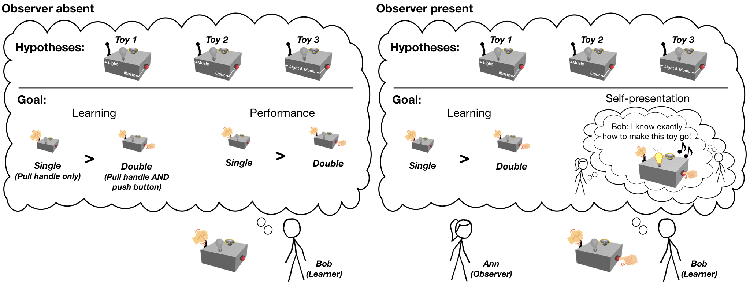
\includegraphics[width=0.95\linewidth]{figs/model_diagram-1} 

}

\caption[Diagram of the computational model]{Diagram of the computational model: The learner considers possible hypotheses and his contextual goals. When an observer is absent, he considers his learning goal (to maximize information gain) and performance goal (e.g. to play music) and decides on an action. When an observer is present, his decision for an action is based on his learning goal vs. presentational goal (to have the observer infer his competence).}\label{fig:model_diagram}
\end{figure*}
\end{CodeChunk}

Work on exploratory actions in active learning often isolates
information goals by removing the learner from any kind of social
context. In contrast, real-world learning is characterized by situations
where there are teachers, peer learners, or other individuals who can
directly influence the utility of information gathering actions. In
fact, a large body of evidence suggests that social reasoning processes
shapes how we learn from evidence. For example, children learn faster
when observing intentional (more informative) actions compared to
accidental (less informative) actions. Moreover, adults and children
will make even stronger inferences if they believe that another person
selected their actions with the goal of helping them learn (i.e.,
teaching) (Shafto, Goodman, \& Frank, 2012).

Models of active learning are not typically able to accommodate these
richer inferences and richer utility structures where people must
integrate the value of social goals -- looking competent or
knowledgeable, for example -- and information goals when deciding what
to do next. Moreover, actions that maximize learning are inherently
risky, and thus are more difficult to undertake in with someone else
present. How can active learning models be modified to accommodate this
richer set of utilities? As a step towards answering this question, we
model a learner who considers a mixture of learning and performance
goals. We assume that these goals are triggered by features of the
social context such as the presence of another individual whom we want
to impress.

We instantiate the predictions of our model in a simple causal learning
task and measure adults' decisions about whether to take actions that
support learning vs.~social goals. We show that emphasizing performance
or self-presentation goals leads to actions that reduce the chances of
learning (E1). Next, we show that the presence of an observer (i.e., a
boss) pushes learners to emphasize performance/presentation actions even
when emphasis is placed on a learning goal (E2). Finally, we present
Bayesian Data Analysis showing that the empirical results are consistent
with predictions of our cognitive model of social-active learning.

\section{Computational model}\label{computational-model}

To examine people's learning-performance tradeoff, we situated our model
and paradigm in a simple learning environment. The learner in our model
has a toy that he can act on, and can choose between two kinds of
actions that will each lead to one outcome (new discovery) or the other
(immediate reward). The learner's action rests on his goals to explore
versus exploit, which in turn are determined in part by the presence or
absence of another person he cares about (i.e.~his
boss)\footnote{From here on, we use a male pronoun for Bob, the learner, and female pronoun for Ann, the boss and observer.}.

A key assumption underlying inferences in recent Bayesian models of
human social cognition is that people act approximately optimally given
a utility function (e.g. Goodman \& Frank, 2016; Jara-Ettinger, Gweon,
Schulz, \& Tenenbaum, 2016). Our model adopts the same utility-theoretic
approach, and assumes an approximately optimal agent who reasons about
the utility function that represents a weighted combination of multiple
goals (Yoon, Tessler, Goodman, \& Frank, 2017). Our model thus reflects
a principled tradeoff between different goals that a learner has in a
social learning context. Specifically, we model how a person may make a
decision to act based on his desire to learn how a toy works
(\emph{learning utility}), to make the toy operate and perform a given
function (\emph{performance utility}), or to present himself as a
competent individual who knows how to make the toy work
(\emph{presentational utility}; see the model diagram in Figure 1).

First, the \emph{learning utility} symbolizes the goal to learn new
information, which in our paradigm specifically is associated with
figuring out how a given toy works. The learning utility is formally
represented by an OED model (Lindley, 1956; ``Optimal Experiment
Design''; Nelson, 2005), which quantifies the \emph{expected utility} of
different information seeking actions. Here we follow the mathematical
details of the OED approach as outlined in Coenen, Nelson, \& Gureckis
(2017) that was implemented in our model. The set of queries, each
realized through taking an action, is defined as
\(Q_1, Q_2, ..., Q_n = {Q}\). The expected utility of each query
(\(EU(Q)\)) is a function of two factors: (1) the probability of
obtaining a specific answer \(P(a)\) weighted by (2) the usefulness of
that answer for achieving the learning goal \(U(a)\).

\[EU(Q) = \sum_{a\in q}{P(a)U(a)}\]

There are a variety of ways to define the usefulness function to score
each answer (for a detailed analysis of different approaches, see Nelson
(2005)). One standard method is to use \emph{information gain}, which is
defined as the change in the learner's overall uncertainty (difference
in entropy) before and after receiving an answer. This information gain
is then the usefulness of the answer to the query, and thus is equal to
the learning utility (\(U_{learn}\)):

\[ U_{learn} = U(a) = \frac{ent(H) - ent(H|a)}{log_2n}\] \noindent
where \(ent(H)\) is defined using Shannon
entropy\footnote{Shannon entropy is a measure of unpredictability or amount of uncertainty in the learner's probability distribution over hypotheses. Intuitively, higher entropy distributions are more uncertain and harder to predict. For example, if the learner believes that all hypotheses are equally likely, then they are in a state of high uncertainty/entropy. In contrast, if the learner firmly believes in one hypothesis, then uncertainty/entropy is low.}.
MacKay (2003), which provides a measure of the overall amount of
uncertainty in the learner's beliefs about the candidate hypotheses.

\[ent(H) = -\sum_{a\in A}{P(h)log_2P(h)}\] \noindent
The conditional entropy computation is the same, but takes into account
the change in the learner's beliefs after seeing an answer.

\[ ent(H|a) = -\sum_{h\in H}{P(h|a)logP(h|a)} \] \noindent
To calculate the change in the learner's belief in a hypothesis
\(P(h|a)\), we use Bayes rule.

\[ P(h|a) = \frac{P(h)P(a|h)}{P(a)} \]

\noindent
Finally, the difference in entropy is normalized by \(log_2 n\).

The learner performs the expected utility computation for each query in
the set of possible queries and picks the one that maximizes utility. In
practice, the learner considers each possible answer, scores the answer
with the usefulness function, and weights the score using the
probability of getting that answer. In our paradigm, a learner thinking
about the learning utility considers acting on the toy one way over
another, and computes how informative a given answer should be in
reducing uncertainty about how the toy works.

Second, the \emph{performance utility} is the utility of successfully
making the toy operate and achieving an immediate rewarding outcome.
Specifically within our current paradigm, the performance utility
(\(U_{perf}\)) is the expected likelihood of performance (e.g.~turning
on music; \(m\)) given the learner's action \(a\).

\[ U_{perf} = P_L(m | a) \] \noindent
Thus, performance utility is maximized by taking an action that is most
likely to make the toy ``go'' and play music or turn the light on, which
is the outcome of interest.

When there is no observer present, the learner considers the tradeoff
between the learning utility and performance utility, and he determines
his action based on a weighted combination of the two utilities:

\[ U(a;\phi; obs = no) = \phi_{learn} \cdot U_{learn} + \phi_{perf} \cdot U_{perf} ,\]
\noindent
where \(\phi\) is a mixture parameter governing the extent to which the
learner prioritizes information gain over immediate reward.

When there is another person present to observe the learner's action,
this observer \(O\) is expected to reason about the competence \(c\) of
the learner \(L\) which is equal to whether the learner was able to make
the toy produce an effect.

\[ P_O(c) \propto P_L(m | a)\]

The learner thinks about how the observer infers the learner's
competence, and his \emph{presentational} utility (\(U_{pres}\))is based
on maximizing the apparent competence inferred by the observer.

\[ U_{pres} = P_O(c) \] When there is an observer present, the learner
considers the tradeoff between all three utilities: the learning
utility, performance utility and presentational utility:

\[ U(m;a;\phi; obs = yes) = \phi_{learn} \cdot U_{learn} + \\ \phi_{perf} \cdot U_{perf} + \phi_{pres} \cdot U_{pres}\]
Based on the utility functions above, the learner (\(L\)) chooses his
action \(a\) approximately optimally (as per optimality parameter
\(\lambda\)) given his goal weight and observer presence.

\[ P_L(a | \phi, obs) \propto \exp(\lambda \cdot \mathbb{E}[U(a;\phi; obs)])\]

\section{Experiment 1}\label{experiment-1}

\begin{CodeChunk}
\begin{figure*}[tb]

{\centering 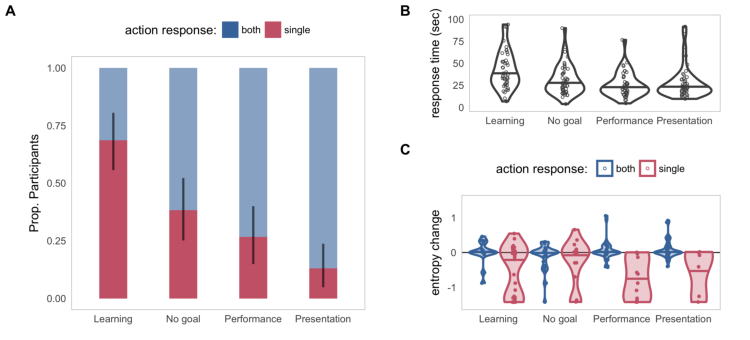
\includegraphics[width=0.95\linewidth]{figs/e1_behav_results_plot-1} 

}

\caption[Behavioral results for E1]{Behavioral results for E1. Panel A shows the proportion of action decisions for each goal condition. Error bars represent 95\% binomial confidence intervals computed using Bayesian inference. Panel B shows violin plots of participants' response times on the action decisions. Each point represents a participant with the width of the violin representing the density of the data at that value. Panel C shows violin plots of participants' belief change (entropy) as a function of condition. Lower values represent higher certainty after selecting an action. Color in panels A and C represent the type of action participants selected.}\label{fig:e1_behav_results_plot}
\end{figure*}
\end{CodeChunk}

In Experiment 1, we first wanted to confirm that participants would
choose different actions depending on the kind of goal that was
highlighted. We were also interested in how people would act when no
goal was specified. Importantly, participants were limited to selecting
a single action, which meant the opportunity cost for the alternative
action was at its highest. Specifically, participants were asked to
imagine that they needed to act on a toy with an uncertain causal
mechanism, and we assigned them to different goal conditions: (1)
learning (``learn how the toy works''), (2) performance (``make the toy
play music''), (3) presentation (``impress their boss''), and (4) no
goal specified.

We hypothesized that participants would choose an informative action
more often in the following order of goal conditions (decreasing):
learning, no goal, performance, and
presentation\footnote{Our hypothesis and method were pre-registered prior to data collection on the Open Science Framework (https://osf.io/kcjau)}.

\subsection{Method}\label{method}

\subsubsection{Participants}\label{participants}

We recruited 196 participants (roughly 50 for each condition) on
Amazon's Mechanical Turk. To participate participants were required to
have an IP addresses in the United States and a task approval rate above
85\%. We excluded 7 participants who failed to answer at least two out
of three manipulation check questions correctly (see Procedure section
for details on the manipulation check), and thus the remaining 189
participants were included in our final analysis.

\subsubsection{Stimuli and Design}\label{stimuli-and-design}

We presented images of three different toys that look very similar but
each work in different ways, and provided instructions for them (see top
of Fig. 1 for what the toys looked like).

\begin{itemize}
\item
  Toy 1: \emph{``Pull the handle on the left to turn on the light. Press
  the button on the right to play music. Doing both produces both
  effects at the same time.''}
\item
  Toy 2: \emph{``Pull the handle on the left to play music. Press the
  button on the right to turn on the light. Doing both produces both
  effects at the same time.''}
\item
  Toy 3: \emph{``Pull the handle on the left AND press the button on the
  right to turn on the light and play music at the same time. The button
  press or handle pull on its own doesn't produce any effect.''}
\end{itemize}

Thus, doing both button press and handle pull was immediately rewarding
but uninformative (as it does not disambiguate the causal mechanism in
any way), whereas either of the single actions was completely
disambiguating, but was uncertain to produce an immediate outcome. Each
toy had a label at the front, indicating which action(s) will make the
toy operate, and with which outcome effect.

We asked participants to act on one of these toys; importantly, the
given toy was missing its label, such that partcipants could not know
whether the toy was Toy 1, 2 or 3. We assigned participants into four
goal conditions. For participants in \emph{learning},
\emph{performance}, and \emph{presentation} conditions,we asked them to
imagine that they were children's toy developers and that one day their
boss approached them. We then instructed participants to: figure out the
correct label for the toy (\emph{learning} condition); make the toy play
music (or turn the light on; \emph{performance} condition); or impress
their boss and show that they are competent (\emph{presentation}
condition). In \emph{no-goal} condition, participants were asked to
select an action. We asked participants to select an action they would
like to try out on the toy in order to accomplish the specified goal,
out of three possible actions: to ``press the button'', ``pull the
handle'', or ``press the button and pull the handle.'' We randomly
assigned each participant to one of the three goal conditions, and
randomized the order of actions to choose from.

\subsubsection{Procedure}\label{procedure}

We first introduced participants to the task, and showed them a picture
of a possible toy with labels on its different parts. Then they read
instructions for each of the three toy types. We presented Toy 1 and Toy
2 instructions in a randomized order first, and then Toy 3 instructions.
Afterwards, they were asked what they would do to make the toy operate
as manipulation check (e.g. ``How would you make the toy play music?'').
We asked participants to rate prior likelihood that an unknown toy is
Toy 1, 2, or 3, to use as priors for our model. Participants then read a
scenario for one of the three goal conditions, followed by the question:
``If you only had one chance to try a SINGLE action to {[}pursue the
specified goal{]}, which action would you want to take? You will get a
10 cent bonus \ldots{} if you {[}achieve the given goal{]}.'' After
selecting one of three possible actions to perform on the toy and seeing
that the toy successfully played music, participants were asked again to
rate the likelihood that the unlabeled toy was each of the three
possible toys.

\subsection{Results and discussion}\label{results-and-discussion}

\subsubsection{Analysis plan}\label{analysis-plan}

First, we present behavioral analyses of participants' (1) action
decisions, (2) action decision times, and (3) belief change (i.e.,
learning).\footnote{See (\url{https://osf.io/kcjau}) for a
  pre-registration of the analysis plan.} Decision times correspond to
the latency to make an action selection as measured from the start of
the action decision trial (all RTs were analyzed in log space). We
quantified participants' beliefs about the possible toy designs using
entropy, and belief change was measured as the difference in entropy
before and after selecting an action.

We used the \texttt{rstanarm} (Gabry \& Goodrich, 2016) package to fit
Bayesian regression models estimating the differences across conditions.
We report the uncertainty in our point estimates using 95\% Highest
Density Intervals (HDI). The HDI provides a range of credible values
given the data and model. All analysis code for the statistical models
can be found in the online repository for this project:
\url{https://github.com/kemacdonald/soc-info/R/03_models.Rmd}.

\subsubsection{Action decisions:}\label{action-decisions}

We modeled action decisions using a logistic regression specified as
\texttt{$action \sim goal\_condition$} with the No-Goal condition as the
reference category. Participants' tendency to select a ``single'' action
varied across conditions in the predicted pattern (see Panel A of Fig
2), with the highest proportion occuring in the Learning context
(\(M_{learn} =\) 68\%, {[}55\%, 80\%{]}), followed by the No Goal
context (\(M_{noGoal} =\) 38\%, {[}25\%, 52\%{]}), then Performance
(\(M_{perform} =\) 27\%, {[}15\%, 40\%{]}), and the fewest single
actions in the Presentation condtion (\(M_{present} =\) 14\%, {[}6\%,
25\%{]}).

Compared to the No-Goal condition, participants selected the single
action at a greater rate in the Learning condition (\(\beta\) = 1.28,
{[}0.5, 2.17{]}) and at lower rate in the Presentation context
(\(\beta\) = -1.41, {[}-2.47, -0.4{]}), with the null value of zero
difference condition falling well outside the 95\% HDI, and at similar
rate in the Performance condition (\(\beta\) = -0.53, {[}-1.43, 0.35{]})
with the 95\% HDI including the null.

\subsubsection{Action decision times:}\label{action-decision-times}

We analyzed response times in log space using the same model
specification. Panel A of Figure 2 shows the full RT data distribution.
On average, participants took 31 seconds to generate a response in the
No-goal condidition. Participants took on on average 12.2 seconds
{[}4.2, 20{]} longer to generate a decision in the Learning condition,
but produced similar response times in the Performance (\(M_{perform}\)
= 27.5, {[}21.9, 33.3{]}) and Presentation (\(M_{present}\) = 27.5,
{[}37.9, 33.2{]}) conditions.

\subsubsection{Belief change:}\label{belief-change}

We modeled change in entropy as a function of goal condition and
participants' action selections:
\texttt{$entropy\_change \sim goal\_condition + action\_response$} (see
Panel C of Fig 2) . Across all conditions, people who selected the
single action showed a greater reduction in entropy (\(\beta\) = -0.49,
{[}-0.64, -0.33{]}, i.e., learned more from their action. We did not see
evidence of an interaction between goal condition and action selection.
However, recall that a larger proportion of participants selected the
single action in the Learning context, so the probability of learning is
higher in this scenario.

\section{Experiment 2}\label{experiment-2}

\begin{CodeChunk}
\begin{figure*}[tb]

{\centering 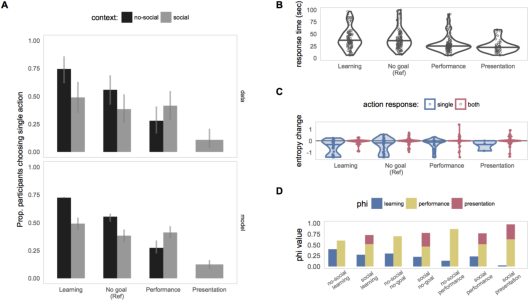
\includegraphics[width=0.95\linewidth]{figs/e2_results-1} 

}

\caption[Behavioral and model fitting results for E2]{Behavioral and model fitting results for E2. Panel A shows actions decisions with color representing social context, from human data (top) and fitted model predictions (bottom). Panel B shows decision times. Panel C shows belief change. Panel D shows inferred phi values for each goal-context condition. All other plotting conventions are the same as Figure 2.}\label{fig:e2_results}
\end{figure*}
\end{CodeChunk}

In Experiment 1, we saw that participants made different action choices
depending on the goal conditions, as we previously predicted. In
Experiment 2, we manipulated goals as well as social contexts, fully
crossing the different goal conditions with the presence/absence of the
boss, to see whether the social context affects people's decision making
differently in each goal condition.

We hypothesized that social pressure should increase
presentation-oriented, immediately-rewarding actions in the learning and
no-goal conditions, but not in the performance condition in which they
are already specified a goal in the same direction.

\subsection{Method}\label{method-1}

\subsubsection{Participants}\label{participants-1}

We recruited 347 participants (\textasciitilde{}50 for each condition)
on Amazon's Mechanical Turk. To participate participants were required
to have an IP addresses in the United States and a task approval rate
above 85\%. We excluded 22 participants who failed to answer at least
two out of three manipulation check questions correctly, and thus the
remaining 325 participants were included in our final analysis.

\subsubsection{Stimuli and Design}\label{stimuli-and-design-1}

The stimuli and design were identical to Experiment 1, except we had
seven different goal \(\times\) social conditions. Goals remained
identical to ones presented in Experiment 1; social conditions varied
depending on whether the boss was present in the story (\emph{social})
or she was absent (\emph{no-social}). Thus, the conditions from
Experiment 1 were used as \emph{social-learning},
\emph{social-performance}, \emph{social-presentation}, and
\emph{no-social-no-goal} conditions in Experiment 2. We added three more
conditions: \emph{no-social-learning}, \emph{no-social-performance}, and
\emph{social-no-goal}. Note that we did not have
\emph{no-social-presentation} condition, because presentation goal by
definition was to present oneself as competent to and impress another
person.

\subsubsection{Procedure}\label{procedure-1}

The procedure was identical to Experiment 1.

\subsection{Results and discussion}\label{results-and-discussion-1}

\subsubsection{Action decisions:}\label{action-decisions-1}

We modeled action decisions using a logistic regression specified as
\texttt{$action \sim goal\_condition * social\_context$} with the
No-Goal and No-Social condition as the reference category. We replicated
the key finding from E1: participants tended to select the ``single''
action more often when they were within a context that emphasized a
learning goal (\(M_{learn} =\) 68\%, {[}57\%, 78\%{]}), followed by the
No Goal context (\(M_{noGoal} =\) 52\%, {[}41\%, 63\%{]}), then
Performance (\(M_{perform} =\) 37\%, {[}26\%, 48\%{]}), with the fewest
single actions generated in the Presentation condtion (\(M_{present} =\)
8\%, {[}2\%, 17\%{]}).

There was a main efffect of social context, with participants being less
likely to select the single action when their boss was present
(\(\beta =\) -0.521, {[}-1.005, -0.053{]}). Finally, there was evidence
for a reliable interaction between goal condition and social context
such that the effect of social context was present in the Learning and
No-Goal conditions, but not in the Performance condition (\(\beta\)
\(_{int}\) = 1.163, {[}0.01, 2.312{]}).

\subsubsection{Action decision times:}\label{action-decision-times-1}

We replicated the key decision time finding from E1: slower decision
times in the Learning context. On average, participants took seconds to
generate a response in the No-goal condidition and seconds in the
Learning condition. In contrast, decisions were faster in the
Performance (\(\beta\) = -7.78 sec, {[}-14.01, -1.52{]}) and
Presentation (-10.77 seconds, {[}-18.67, -2.73{]}) conditions, which
were similar to one another (see Panel B of Fig 3). There was no
evidence of a main effect of social context or an interaction between
goal condition and social context. Note that we did not see a difference
in decision times between the Learning and No-Goal conditions, which is
different from the pattern in E1.

\subsubsection{Belief change:}\label{belief-change-1}

Across all conditions, participants who selected the single action
showed a greater reduction in entropy (\(\beta\) = -0.35, {[}-0.45,
-0.24{]}. There was some (weaker) evidence of greater reduction in
entropy in the Learning goal condition (\(\beta\) = -0.12, {[}-0.25,
0.01). There was no evidence of a main effect of social context and no
two- or three-way interactions between social context, goal condition,
and type of action choice.

\subsubsection{BDA model-data fit:}\label{bda-model-data-fit}

In this experiment, participants were instructed to choose an
action\footnote{For action priors, we used a separate prior elicitation task, in which people indicated the likelihood for selecting an action without any background information about possible hypotheses or goals. The results suggested that none of the action choice priors differed from chance. We used mean likelihood for each action choice as baseline priors in our model; see [FIXME]}
based on a certain goal. We assumed that the goal descriptions (e.g.
``figure out the correct label for the toy'') conveyed to the
participants a particular set of goal weights \{\(\phi_{learn}\),
\(\phi_{perf}\), \(\phi_{pres}\)\} that they used to generate their
action choices. We put uninformative priors on these weights
(\(\phi \sim Uniform(0,1)\)) and inferred their credible values
separately for each pair of different goal condition and social context,
using Bayesian data analytic techniques (Lee \& Wagenmakers, 2014).

The inferred goal weights were consistent with what we predicted (see
Figure 3, panel D). \(\phi_{learn}\) was at its highest for no-social
learning condition, in which the goal to learn was highlighted, and
there was minimum social pressure. On the other hand, the
\(\phi_{perf}\) and \(\phi_{pres}\) together make up the highest portion
in the presentation condition, with high social pressure to present
competence, compared to other conditions.

We also inferred another parameter of the cognitive model, the
optimality parameter \(\lambda\). We put uninformative prior on the
parameter (\(\lambda \sim Uniform(0,10)\) and inferred its posterior
credible value from the data. We ran 4 MCMC chains for 100,000
iterations, discarding the first 50,000 for burnin. The Maximum A-
Posteriori (MAP) estimate and 95\% Highest Probability Density Interval
(HDI) for \(\lambda\) was 4.79 {[}3.96, 6.2{]}.

The predictions of the action choices according to the fitted learner
model are shown in Figure 3, panel A (bottom). The model's expected
posteriors over action choices capture key differences between
conditions: the single action was more likely for no-social than social
conditions overall, but not when the performance goal was highlighted.
The model was able to predict the distribution of action responses with
high accuracy \(r^2(21)\) = 0.9.

\section{General Discussion}\label{general-discussion}

How does the social context shape our decision making in an active
learning environment? We proposed that people make decisions based on a
principled tradeoff between learning- and performance-oriented goals,
and that the social context influences the desire to present oneself as
competent and knowledgeable, and may encourage pursuit of immediate
effect outcome. In two experiments, we confirmed that people's behaviors
were in line with our hypothesis, as they chose more informative actions
when learning goals were highlighted with no boss present, while they
chose more immediately rewarding actions when performance or
presentational goals were highlighted, especially when the boss was
present on scene. When no goal was specified, people showed behavior
that seemed to reflect a mix of the goals in tradeoff. Our computational
model successfully captured key patterns in these behavioral data.

Our model has implications for many interesting future directions. For
example, how might attitudes toward learning and social goals change at
different time points? How do people behave differently for verbal
question-asking to seek knowledge; how would people decide whether or
not to ask for new information, at the risk of appearing ignorant? How
does the ability to balance between learning versus self-presentation
goals emerge and develop? What is an ``optimal'' learning environment,
that is, what balance of informational and social goals promote the most
effective learning? Our work represents the first step to answering
these questions that ultimately seek to unify theories on active
learning and social reasoning.

\section{Acknowledgements}\label{acknowledgements}

This work was supported by NSERC postgraduate doctoral scholarship
PGSD3-454094-2014 to EJY and an NSF GRFP to KM {[}FIXME{]}.

\section{References}\label{references}

\setlength{\parindent}{-0.1in} \setlength{\leftskip}{0.125in} \noindent

\hypertarget{refs}{}
\hypertarget{ref-castro2009human}{}
Castro, R. M., Kalish, C., Nowak, R., Qian, R., Rogers, T., \& Zhu, X.
(2009). Human active learning. In \emph{Advances in neural information
processing systems} (pp. 241--248).

\hypertarget{ref-coenen2017}{}
Coenen, A., Nelson, J. D., \& Gureckis, T. M. (2017). Asking the right
questions about human inquiry.

\hypertarget{ref-gabry2016rstanarm}{}
Gabry, J., \& Goodrich, B. (2016). Rstanarm: Bayesian applied regression
modeling via stan. r package version 2.10. 0.

\hypertarget{ref-goodman2016}{}
Goodman, N. D., \& Frank, M. C. (2016). Pragmatic language
interpretation as probabilistic inference. \emph{Trends in Cognitive
Sciences}, \emph{20}(11), 818--829.

\hypertarget{ref-grabinger1995rich}{}
Grabinger, R. S., \& Dunlap, J. C. (1995). Rich environments for active
learning: A definition. \emph{ALT-J}, \emph{3}(2), 5--34.

\hypertarget{ref-jara2016}{}
Jara-Ettinger, J., Gweon, H., Schulz, L. E., \& Tenenbaum, J. B. (2016).
The naïve utility calculus: Computational principles underlying
commonsense psychology. \emph{Trends in Cognitive Sciences},
\emph{20}(8), 589--604.

\hypertarget{ref-lee2014bayesian}{}
Lee, M. D., \& Wagenmakers, E.-J. (2014). \emph{Bayesian cognitive
modeling: A practical course}. Cambridge university press.

\hypertarget{ref-lindley1956}{}
Lindley, D. V. (1956). On a measure of the information provided by an
experiment. \emph{The Annals of Mathematical Statistics}, 986--1005.

\hypertarget{ref-mackay2003}{}
MacKay, D. J. (2003). \emph{Information theory, inference and learning
algorithms}. Cambridge university press.

\hypertarget{ref-nelson2005}{}
Nelson, J. D. (2005). Finding useful questions: On bayesian
diagnosticity, probability, impact, and information gain.
\emph{Psychological Review}, \emph{112}(4).

\hypertarget{ref-settles2012active}{}
Settles, B. (2012). Active learning. \emph{Synthesis Lectures on
Artificial Intelligence and Machine Learning}, \emph{6}(1), 1--114.

\hypertarget{ref-shafto2012learning}{}
Shafto, P., Goodman, N. D., \& Frank, M. C. (2012). Learning from
others: The consequences of psychological reasoning for human learning.
\emph{Perspectives on Psychological Science}, \emph{7}(4), 341--351.

\hypertarget{ref-sutton1998}{}
Sutton, R. S., \& Barto, A. G. (1998). \emph{Introduction to
reinforcement learning} (Vol. 135). MIT Press Cambridge.

\hypertarget{ref-yoon2017}{}
Yoon, E. J., Tessler, M. H., Goodman, N. D., \& Frank, M. C. (2017). ``I
won't lie, it wasn't amazing'': Modeling polite indirect speech. In
\emph{Proceedings of the thirty-ninth annual conference of the Cognitive
Science Society}.

\end{document}
